\section{Software Side}
\label{sec:software_side}
\subsection{Software Components}

The latest published software stack of YouTube is from 2012, when the head architect Mike Solomon gave a speech about the Scalibility of YouTube \cite{misc:scalibility_at_youtube} \cite{misc:hihgscalibility}. In Table~\vref{tab:software_components} the most important components mentioned by Solomon are listed.

\begin{table}[htbp]
  \begin{center}
    \begin{tabularx}{\textwidth}{|p{0.2\textwidth}|p{0.35\textwidth}|X|}
      \hline
      \textbf{Software \newline Component} & \textbf{Role} & \textbf{Reasons for usage} \newline (given in Solomon's speech) \\
      \hline
      \hline
      Linux & Operating system for web and cache servers & There is always a way to check the behaviour of the system - no matter how bad the application is written, at some fundamental level the resources its consuming are explorable \\
      \hline
      Apache \newline HTTP Server & HTTP Server - every video request goes through Apache & Not mentioned \\
      \hline
      MySQL & Database for - among others - the videos & Depending on the use case, the configuration and the right queries it can scale very well \\
      \hline
      Vitess & Front-end for MySQL - it serves every YouTube database request & Mainly query optimizations and rewriting \\
      \hline
      Apache Zookeeper & Distributed lock server, massively used for distributed configurations & Not mentioned \\
      \hline
    \end{tabularx}
    \caption{Software Components for YouTube servers}
    \label{tab:software_components}
  \end{center}
\end{table}

It is remarkable that YouTube uses a lot of tools which are also used by smaller companies with much smaller web traffic. This is because their main programming/architecture goal is to keep everything as simple as possible as long as it works properly and scales. Thereby they also keep their flexibility to solve current and future problems.\\
\\
For the same reasons, YouTube is using Python as its main programming language to handle video requests. Performance-wise code written in Python is generally worse than similiar code written in languages like C, but new demands can be served much faster in most cases, which is more important for constantly changing (web) applications like YouTube.

\subsection{Scalability Techniques}

Solomon also mentioned in his speech the different kinds of high-level scalability techniques which are used by YouTube to handle the enormous traffic:

\begin{description}
  \item[Divide \& Conquer:] The most used general scalibilty technique, where everything possible is partioned out. This includes among others the ability to add new web and cache servers to the cache clusters to manage bigger traffic.

  \item[Approximate correctness:] The global state of the YouTube system can be inconsistent. It only matters, whether the user recognizes these inconsistency. For example a user who writes a comment immediately wants to see the comment, but another user who watches the respective video does not care about the comment, because he does not know about it. Thus the system does not have to have globally consistent transactions, which would be very expensive. YouTube does not trigger a single transaction for a single comment, they rather update the comments in their system from time to time.

  \item[Jitter - Add entropy to the system:] Adding entropy to a large dis\-tri\-bu\-ted system can help to avoid so called thundering herds. For example if every cache server would have the same cache expiration time for a popular video, a thundering herd could be created, because all servers would expire the video at the same time. The solution in this case is to add entropy by setting the expiration time randomly in a specific time frame.
\end{description}

The approximation of the correctness is noteworthy, because YouTube does not guarentee a user who is watching a video that the comments, the view counter and the like/dislike counter are up to date. This is pretty different in comparison to business applications, where global consistency is very important. Moreover without this kind of cheating the scalibility of the YouTube web page would be probably much worse.

\subsection{Traffic Management}

YouTube videos are requested via HTTP over TCP, which is a transport protocol that assures reliable transfer by retransmitting lost data packets and performs congestion control to avoid overloading the network. As observed by \cite{inc:transport_protocols}, watching YouTube videos over UDP is also possible, but can result in visual impairments of the video contents if there is a network bottleneck. TCP on the other hand may lead to stalling of the video stream, but still outperforms UDP regarding Quality of Experience due to the paper. \\
\\
YouTubes delivery strategy has been studied in great detail by Rao \emph{et al.} \cite{inp:network_characteristics}, where they show, that the respective strategy mainly depends on the factors listed in Table~\vref{tab:depence_factors}.

\begin{table}[htbp]
  \begin{center}
    \begin{tabularx}{\textwidth}{|l|X|}
      \hline
      \textbf{Dependence factor} & \textbf{Example} \\
      \hline
      \hline
      The video container & Flash plugin or HTML5 container \\
      \hline
      The type of client device & Desktop or mobile devices \\
      \hline 
      Type of browser & Google Chrome, Mozilla Firefox, Internet Explorer, Safari etc. \\
      \hline
    \end{tabularx}
    \caption{Dependence factors of the delivery strategy}
    \label{tab:depence_factors}
  \end{center}
\end{table}

Considering these factors, the strategies primarily differ in two video content transferring phases - the \textbf{buffering state phase} and \textbf{steady state phase}. They are illustrated in Figure~\vref{fig:transferring_phases}.

\begin{figure}[htbp]
  \begin{minipage}{\textwidth}
    \begin{center}
      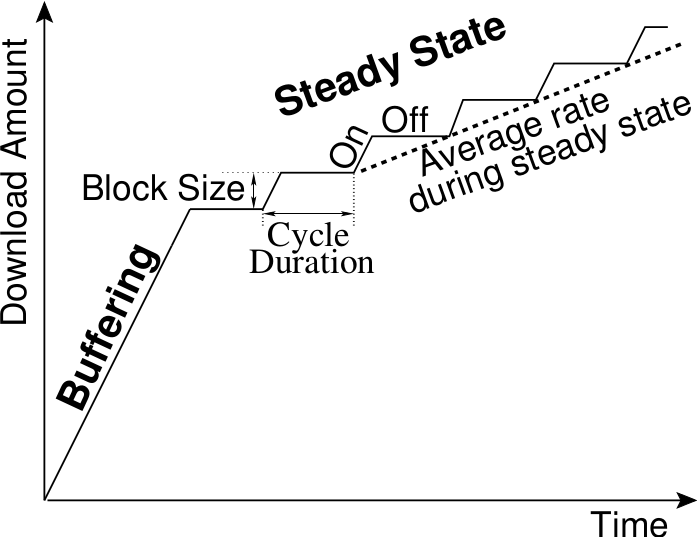
\includegraphics[width=0.5\textwidth]{pictures/transferring_phases.png}
      \caption[test]{YouTube video content transferring phases\footnotemark[2]}
    \label{fig:transferring_phases}
    \end{center}
  \end{minipage}
\end{figure}

\footnotetext[2]{Taken from \cite{inp:network_characteristics}}

\begin{description}
  \item[Buffering phase:] In this phase the video will not be played first, but the initial video content part will be downloaded, which is called buffering. Thereby the data transfer rate is limited by the available end-to-end bandwidth. The playback begins when an efficient amount of data is available is in its buffer.

  \item[Steady state phase:] In this phase the video is tried to be playbacked with preferably few interruptions. In the best case the average download rate in slightly larger than the video encoding. If the average download rate gets smaller then the encoding rate, there will be interruptions in the playback of the video. The average download rate in  is achieved by periodically transferring one block of video content. These periodic transfers produce cycles of ON-OFF periods. During each ON period, a block of data is transferred at the end-to-end available bandwidth that can be used by TCP; the TCP connection is idle during the OFF periods.
\end{description}

The smooth playback of all videos for all users is a very important goal for YouTube to ensure the Quality of Experience. Besides this, they try to avoid transmitting to much data in advance of consumption in order to reduce the amount of buffering at the client, which is particularly relevant in the case of mobile devices and to reduce the waste of network and server resources by sending data that are never used. As to that Finamore \emph{et al.} \cite{inpr:youtube_everywhere} observed that people tend to abort the playback very soon, with 60\% of videos being watched for less than 20\% of their duration, which results in 25\%-39\% of data transferred unnecessarily. This waste of network traffic is even higher when mobile devices are considered. YouTube is well aware of these facts and therefore aggressive buffering is performed when a video is requested. This means that initially during the buffering phase the server sends as fast as possible to fill up the initial client buffer \cite{inp:network_characteristics}. When about 40 seconds of the video are loaded, the steady state phase will begin. Thus an initial smooth playback can be reached.


